% alloptions=yes
\RCS $Revision$
\begin{aufgabe}[Technologie]{Messschieber}
   \begin{teilaufgabe}[ohnenummer]{t}{0}{2}
       Nach dem Messen mit einem Messschieber erhält man die abgebildeten
       Anzeigewerte. Lesen Sie das genaue Maß ab. \par
       \vspace{5mm} \par
       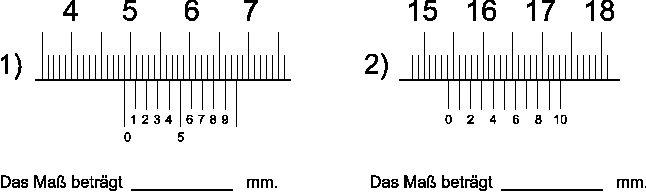
\includegraphics[width=155mm]{aufgabe-2} \par
   \end{teilaufgabe}
   \begin{loesung}
       \punkte[32,3]{48,9\,mm}{1}{} 
       \punkte[119,3]{154,1\,mm}{1}{}
   \end{loesung}
\end{aufgabe}

